\section{Methods I: Kinematic position angle analysis}
\label{sec:methods-I-kinemetry}

\subsection{Kinematic PA analysis method description}
\label{kinemetry-analysis-method-description}
% \subsection{Quality screening}
Global kinematic velocity position angles (PA) for the PSB and control galaxy samples were determined using the \texttt{fit\_kinemetry\_pa} routine as described in appendix C of \cite{2006MNRAS.366..787K}. The routine returns the angle of the line bisecting the greatest change in velocity between the receding and approaching sides. \cite{2019MNRAS.483..172D} performed a \texttt{kinemetry} analysis of over 8,000 galaxies from the MaNGA Product Launch MPL-8 internal data release. In order to obtain a clean sample of well defined global PAs they visually classified the stellar and H$\alpha$ gas velocity fields of all galaxies in their sample into 3 categories (Chris Duckworth, 2019, personal communication), and set flags in their dataset as follows:

\begin{itemize}
    \item {Flag 1} : Dominant coherent rotation and well defined PA
    \item {Flag 2} : Dominant coherent rotation but with complex motions or highly inclined velocity fields 
    \item {Flag 3} : Do not use
\end{itemize}

During this analysis galaxies with significant kinematic features such kinematically decoupled cores (KDCs) and warped velocity fields were also identified.

The resulting MPL-8 screened dataset of galaxies with reliable global PAs (flagged as [1] or [2]) from \cite{2019MNRAS.483..172D} was matched with the PSB galaxies in the sample of Chen et al. (2019, in prep.) to obtain a subset of PSBs with good \texttt{kinemetry} analysis flags. Furthermore a subset of those PSBs with $\Delta$PAs \textgreater 30\textdegree\ was extracted. The results are shown in Tables \ref{tab:offsetCPSBs} and \ref{tab:offsetRPSBs}. 

Examples of PSBs with misaligned stellar and gas velocity fields for a CPSB and an RPSB is shown in Figure \ref{fig:alligned-misaligned}. In classical kinematic position angle analysis it is considered significant if the gas and stellar velocity field offset position angle $\Delta$PA$_{k}$ is greater than 30\textdegree. This can be an indication of past disruption of the galaxy.

\begin{figure*}
    \centering
    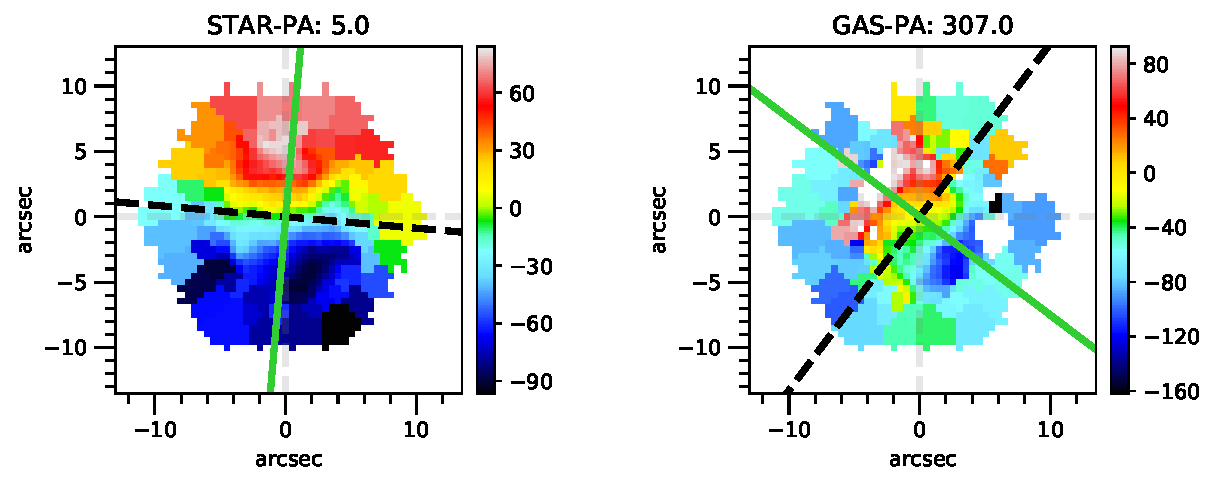
\includegraphics[width=0.8\textwidth]{images/PAplots/PAplotsCPSB/8313-6101-PA.pdf}
    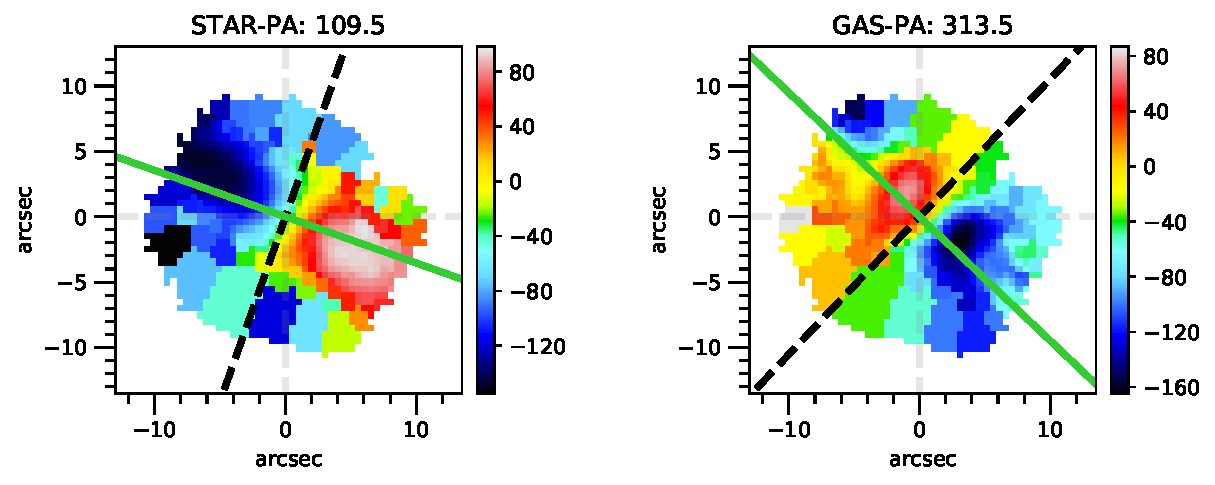
\includegraphics[width=0.8\textwidth]{images/PAplots/PAplotsRPSB/8323-6103-PA.pdf}
    \caption[Examples of PSBs exhibiting significant $\Delta$PA$_{k}$: CPSB 8313-6101 and RPSB 8323-6103.]{This figure is similar to the typical PA$_{k}$ misalignment plots shown in Figure \ref{fig:alligned-misaligned} but provides specific examples for PSBs selected from our sample. The kinematic position angles (PA$_{k}$) for the stellar velocity fields (left) and gas velocity fields (right) are shown for CPSB 8313-6101 (top), and RPSB 8323-6103 (bottom). The velocity field (gas or stars) position angle is displayed as the green solid line while the black dashed line denotes the bisector of the velocity field between the receding (red) and approaching (blue) sides. The velocity colour scale is \kms. Credit for data analysis and plots: Chris Duckworth.}
    \label{fig:CPSB-8313-6101-PA}
\end{figure*}

\subsection{Position angle misalignment}
\label{PA-misalignment}
The gas and velocity field position angle misalignment measurements for PSBs where the $\Delta$PA \textgreater 30\textdegree are tabulated in Figure \ref{tab:offsetCPSBs} for the CPSBs, and Figure \ref{tab:offsetRPSBs} for the RPSBs. Here is can be seen that the number of PSBs galaxies having clearly defined $\Delta$PAs, i.e. \textgreater 30\textdegree, is small fraction of the PSB sample: 5 out of 30 (17\%) CPSBs, and 9 out of 37 (24\%) RPSBs.

\begin{table}
\centering
\caption{CPSBs with gas and stellar velocity kinematic PA offsets \textgreater 30\textdegree.}
\label{tab:offsetCPSBs}
\begin{tabular}{lccc}
\hline
PlateIFU  & Stellar PA & H$\alpha$ PA & $\Delta$PA \\
  & (deg.) & (deg.) & (deg.) \\
\hline
8313-6101 & 5 & 307 & 58 \\
8655-1902 & 335 & 127 & 152 \\
8725-1902 & 22 & 175 & 153 \\
8938-6102 & 214 & 47.5 & 166.5 \\
9494-3701 & 140.5 & 243 & 102.5 \\
\hline
\end{tabular}
\end{table}

\begin{table}
\centering
\caption[RPSBs with kinematic velocity PA offsets \textgreater 30\textdegree.]{RPSBs with gas and stellar velocity kinematic PA offsets \textgreater 30\textdegree.}
\label{tab:offsetRPSBs}
\begin{tabular}{lccc}
\hline
PlateIFU   & Stellar PA & H$\alpha$ PA & $\Delta$PA \\
  & (deg.) & (deg.) & (deg.) \\
\hline
8080-3704 & 24 & 154 & 130 \\
8262-3701 & 153.5 & 118.5 & 35 \\
8323-6103 & 109.5 & 313.5 & 156 \\
8439-6104 & 5.5 & 107 & 101.5 \\
8453-3704 & 44 & 91 & 47 \\
8486-1901 & 295.5 & 85 & 149.5 \\
8554-3701 & 250 & 68 & 178 \\
8932-12704 & 166.5 & 134.5 & 32 \\
9872-3701 & 208.5 & 81 & 127.5 \\
\hline
\end{tabular}
\end{table}

